% Options for packages loaded elsewhere
\PassOptionsToPackage{unicode}{hyperref}
\PassOptionsToPackage{hyphens}{url}
%
\documentclass[
]{book}
\usepackage{lmodern}
\usepackage{amssymb,amsmath}
\usepackage{ifxetex,ifluatex}
\ifnum 0\ifxetex 1\fi\ifluatex 1\fi=0 % if pdftex
  \usepackage[T1]{fontenc}
  \usepackage[utf8]{inputenc}
  \usepackage{textcomp} % provide euro and other symbols
\else % if luatex or xetex
  \usepackage{unicode-math}
  \defaultfontfeatures{Scale=MatchLowercase}
  \defaultfontfeatures[\rmfamily]{Ligatures=TeX,Scale=1}
\fi
% Use upquote if available, for straight quotes in verbatim environments
\IfFileExists{upquote.sty}{\usepackage{upquote}}{}
\IfFileExists{microtype.sty}{% use microtype if available
  \usepackage[]{microtype}
  \UseMicrotypeSet[protrusion]{basicmath} % disable protrusion for tt fonts
}{}
\makeatletter
\@ifundefined{KOMAClassName}{% if non-KOMA class
  \IfFileExists{parskip.sty}{%
    \usepackage{parskip}
  }{% else
    \setlength{\parindent}{0pt}
    \setlength{\parskip}{6pt plus 2pt minus 1pt}}
}{% if KOMA class
  \KOMAoptions{parskip=half}}
\makeatother
\usepackage{xcolor}
\IfFileExists{xurl.sty}{\usepackage{xurl}}{} % add URL line breaks if available
\IfFileExists{bookmark.sty}{\usepackage{bookmark}}{\usepackage{hyperref}}
\hypersetup{
  pdftitle={Mini-Workshop (Structural) Topic Models},
  pdfauthor={Marko Bachl},
  hidelinks,
  pdfcreator={LaTeX via pandoc}}
\urlstyle{same} % disable monospaced font for URLs
\usepackage{color}
\usepackage{fancyvrb}
\newcommand{\VerbBar}{|}
\newcommand{\VERB}{\Verb[commandchars=\\\{\}]}
\DefineVerbatimEnvironment{Highlighting}{Verbatim}{commandchars=\\\{\}}
% Add ',fontsize=\small' for more characters per line
\usepackage{framed}
\definecolor{shadecolor}{RGB}{248,248,248}
\newenvironment{Shaded}{\begin{snugshade}}{\end{snugshade}}
\newcommand{\AlertTok}[1]{\textcolor[rgb]{0.94,0.16,0.16}{#1}}
\newcommand{\AnnotationTok}[1]{\textcolor[rgb]{0.56,0.35,0.01}{\textbf{\textit{#1}}}}
\newcommand{\AttributeTok}[1]{\textcolor[rgb]{0.77,0.63,0.00}{#1}}
\newcommand{\BaseNTok}[1]{\textcolor[rgb]{0.00,0.00,0.81}{#1}}
\newcommand{\BuiltInTok}[1]{#1}
\newcommand{\CharTok}[1]{\textcolor[rgb]{0.31,0.60,0.02}{#1}}
\newcommand{\CommentTok}[1]{\textcolor[rgb]{0.56,0.35,0.01}{\textit{#1}}}
\newcommand{\CommentVarTok}[1]{\textcolor[rgb]{0.56,0.35,0.01}{\textbf{\textit{#1}}}}
\newcommand{\ConstantTok}[1]{\textcolor[rgb]{0.00,0.00,0.00}{#1}}
\newcommand{\ControlFlowTok}[1]{\textcolor[rgb]{0.13,0.29,0.53}{\textbf{#1}}}
\newcommand{\DataTypeTok}[1]{\textcolor[rgb]{0.13,0.29,0.53}{#1}}
\newcommand{\DecValTok}[1]{\textcolor[rgb]{0.00,0.00,0.81}{#1}}
\newcommand{\DocumentationTok}[1]{\textcolor[rgb]{0.56,0.35,0.01}{\textbf{\textit{#1}}}}
\newcommand{\ErrorTok}[1]{\textcolor[rgb]{0.64,0.00,0.00}{\textbf{#1}}}
\newcommand{\ExtensionTok}[1]{#1}
\newcommand{\FloatTok}[1]{\textcolor[rgb]{0.00,0.00,0.81}{#1}}
\newcommand{\FunctionTok}[1]{\textcolor[rgb]{0.00,0.00,0.00}{#1}}
\newcommand{\ImportTok}[1]{#1}
\newcommand{\InformationTok}[1]{\textcolor[rgb]{0.56,0.35,0.01}{\textbf{\textit{#1}}}}
\newcommand{\KeywordTok}[1]{\textcolor[rgb]{0.13,0.29,0.53}{\textbf{#1}}}
\newcommand{\NormalTok}[1]{#1}
\newcommand{\OperatorTok}[1]{\textcolor[rgb]{0.81,0.36,0.00}{\textbf{#1}}}
\newcommand{\OtherTok}[1]{\textcolor[rgb]{0.56,0.35,0.01}{#1}}
\newcommand{\PreprocessorTok}[1]{\textcolor[rgb]{0.56,0.35,0.01}{\textit{#1}}}
\newcommand{\RegionMarkerTok}[1]{#1}
\newcommand{\SpecialCharTok}[1]{\textcolor[rgb]{0.00,0.00,0.00}{#1}}
\newcommand{\SpecialStringTok}[1]{\textcolor[rgb]{0.31,0.60,0.02}{#1}}
\newcommand{\StringTok}[1]{\textcolor[rgb]{0.31,0.60,0.02}{#1}}
\newcommand{\VariableTok}[1]{\textcolor[rgb]{0.00,0.00,0.00}{#1}}
\newcommand{\VerbatimStringTok}[1]{\textcolor[rgb]{0.31,0.60,0.02}{#1}}
\newcommand{\WarningTok}[1]{\textcolor[rgb]{0.56,0.35,0.01}{\textbf{\textit{#1}}}}
\usepackage{longtable,booktabs}
% Correct order of tables after \paragraph or \subparagraph
\usepackage{etoolbox}
\makeatletter
\patchcmd\longtable{\par}{\if@noskipsec\mbox{}\fi\par}{}{}
\makeatother
% Allow footnotes in longtable head/foot
\IfFileExists{footnotehyper.sty}{\usepackage{footnotehyper}}{\usepackage{footnote}}
\makesavenoteenv{longtable}
\usepackage{graphicx,grffile}
\makeatletter
\def\maxwidth{\ifdim\Gin@nat@width>\linewidth\linewidth\else\Gin@nat@width\fi}
\def\maxheight{\ifdim\Gin@nat@height>\textheight\textheight\else\Gin@nat@height\fi}
\makeatother
% Scale images if necessary, so that they will not overflow the page
% margins by default, and it is still possible to overwrite the defaults
% using explicit options in \includegraphics[width, height, ...]{}
\setkeys{Gin}{width=\maxwidth,height=\maxheight,keepaspectratio}
% Set default figure placement to htbp
\makeatletter
\def\fps@figure{htbp}
\makeatother
\setlength{\emergencystretch}{3em} % prevent overfull lines
\providecommand{\tightlist}{%
  \setlength{\itemsep}{0pt}\setlength{\parskip}{0pt}}
\setcounter{secnumdepth}{5}
\usepackage{booktabs}
\usepackage[]{natbib}
\bibliographystyle{apalike}

\title{Mini-Workshop (Structural) Topic Models}
\author{Marko Bachl}
\date{Sommersemester 2020 \textbar{} IJK Hannover}

\begin{document}
\maketitle

{
\setcounter{tocdepth}{1}
\tableofcontents
}
\hypertarget{uxfcberblick}{%
\chapter{Überblick}\label{uxfcberblick}}

\hypertarget{inhalt-des-virtuellen-mini-workshops}{%
\section{Inhalt des virtuellen Mini-Workshops}\label{inhalt-des-virtuellen-mini-workshops}}

\begin{itemize}
\tightlist
\item
  In diesem Mini-Workshop erläutere ich das praktische Vorgehen einer Datenanalyse mit \emph{Structural Topic Models}. Wir behandeln die folgenden Schritte im Analyseprozess:

  \begin{itemize}
  \tightlist
  \item
    Schätzen eines ersten Modells
  \item
    Modellvergleich zur Auswahl eines geeigneten Modells
  \item
    Interpretation der Topics im finalen Modell
  \item
    Darstellung der Ergebnisse
  \item
    Weitere Analysen

    \begin{itemize}
    \tightlist
    \item
      Identifikation verwandter Themen
    \item
      Zusammenhänge der Themenprävalenz mit Kovariaten.
    \end{itemize}
  \end{itemize}
\item
  Wir verwenden das Paket \texttt{\{stm\}} \citep{robertsStmPackageStructural2019} zum Schätzen von Topic Models. Für die Variante der \emph{Structural} Topic Models und die Implementation in diesem Paket sprechen \emph{für mich} die folgenden Gründe

  \begin{itemize}
  \tightlist
  \item
    Gute Integration mit \emph{R} und Paketen, die ich für die Arbeit mit Text-Daten verwende (insbesondere \texttt{\{quanteda\}} und \texttt{\{tidytext\}})
  \item
    Gute ergänzende Pakete zur Arbeit mit den Modellen (insbesondere \texttt{\{stminsights\}})
  \item
    Vergleichsweise schnelle Modellschätzung auch mit großen Datensätzen
  \item
    Direktes Schätzen von Zusammenhängen von Topics mit Kovariaten
  \item
    Initialisieren der Modellschätzung mit dem Spectral Algorithmus
  \item
    Recht weit verbreitet in einem Feld, in dem ich viel lese (Politische Kommunkation nach einem weitem Verständnis)
  \end{itemize}
\item
  Die Darstellung basiert auf einer Analyse, die ich gemeinsam mit Elena Link durchgeführt habe. Wir untersuchten, wie das Thema Impfen in Online-Foren für Eltern diskutiert wurde. Wir verwenden aber nur einen \emph{nicht repräsentativen} Ausschnitt aus dem Material, um die notwendige Rechenleistung und -zeit zu verringern.

  \begin{itemize}
  \tightlist
  \item
    Einen Preprint zur Analyse könnt ihr hier lesen: \href{https://osf.io/ad9h7/}{Vaccine-related Discussions in Online Communities for Parents. A Quantitative Overview}.
  \item
    Die Dokumentation zur Studie ist hier verfügbar: \url{https://bachl.github.io/vaccine_discussions/}. Daten und Analyse-Skripts gibt es im \href{https://osf.io/twx38/}{OSF}. In diesem Material werde auch die Datenerhebung mittels Web-Scraping und die Datenaufbereitung erläutert. Diese Inhalte sind \emph{nicht} Teil dieses Workshops. Wenn ihr Fragen dazu habt, dürft ihr sie natürlich stellen.
  \end{itemize}
\end{itemize}

\hypertarget{welche-inhalte-wir-nicht-behandeln}{%
\section{\texorpdfstring{Welche Inhalte wir \emph{nicht} behandeln}{Welche Inhalte wir nicht behandeln}}\label{welche-inhalte-wir-nicht-behandeln}}

\begin{itemize}
\item
  Auch wenn das im direkten Vergleich mit dem Parallel-Angebot zu \href{https://bachl.github.io/workshop_panel/}{Panel Data Analysis} (meine Ausführlichkeit dort sind ein Grund für die spätere Lieferung dieser Materialien) enttäuschend sein mag: Die Inhalte in diesem Mini-Workshop entsprechen in ihrem Umfang wirklich nur dem, was ich zu Beginn des Digital-Semesters geplant und angekündigt hatte. Der Mini-Workshop ersetzt keine tiefer gehende Einarbeitung in die Methode, sondern ist als ein Einstieg zu verstehen.
\item
  Wir behandeln hier keine theoretischen, statistischen oder auf die Software-Implementierung der Modellschätzung bezogenen Fragen. Die Grundlagen dazu können aus den Texten im LMS entnommen werden \citep{maierApplyingLDATopic2018, robertsStmPackageStructural2019}.
\item
  Es gibt neben \texttt{\{stm\}} viele andere Implementationen in \emph{R} und ihn anderer Software. Gefühlt gibt es alle 6 Monate eine neue Variante von Topic Models, alle 3 Monate eine neue Implementierung und jeden Monat ein Paket mit zusätzlichen Tools für die Arbeit mit Topic Models. Meine Entscheidung für \texttt{\{stm\}} ist keine informierte Entscheidung gegen andere Varianten, Implementierungen und Tools. Dieser Workshop ist keine Aufforderung, ausschließlich \texttt{\{stm\}} zu nutzen. Informiert euch gegebenenfalls selbst über Software-Lösungen, die für eure Bedürfnisse geeignet sind.
\item
  Dieser Mini-Workshop ist kein \emph{R}-Tutorial. Wenn ihr Interesse habt, \emph{R}-Kenntnisse zu erwerben und zu vertiefen, empfehle ich \href{https://r4ds.had.co.nz/}{R4DS}.
\item
  Dieser Mini-Workshop ist keine allgemeine Einführung in die computergestützte Inhaltsanalyse. Wenn ihr allgemein mit \emph{R} arbeiten möchtet, empfehle ich zu diesem Thema die \href{http://inhaltsanalyse-mit-r.de/}{Einführung von Cornelius Puschmann}.
\end{itemize}

\hypertarget{aufbau-des-workshops}{%
\section{Aufbau des Workshops}\label{aufbau-des-workshops}}

\begin{itemize}
\tightlist
\item
  Inhaltlicher Aufbau: Siehe Kapitel-Gliederung
\end{itemize}

\hypertarget{material}{%
\subsection*{Material}\label{material}}
\addcontentsline{toc}{subsection}{Material}

\begin{itemize}
\item
  Dieses Dokument + R Skripte: (Hoffentlich) mehr oder weniger selbsterklärendes Material

  \begin{itemize}
  \tightlist
  \item
    Kuratierte Form ist dieses HTML-Dokument
  \item
    Es gibt auch ein PDF, das ich aber nicht formatiert habe
  \end{itemize}
\item
  Daten: Ein Ausschnitt auf den Daten der oben genannten Beispielstudie. Eine genauere Beschreibung folgt im nächsten Abschnitt.
\item
  Screencast: Zu einigen Analyseschritten stelle ich Screencasts zur Verfügung. Diese sind größtenteils ergänzend gedacht. Bis auf wenige Ausnahmen sollte das schriftliche Material selbsterklärend sein.
\item
  Übungen: Zu einigen Analysen gibt es Übungsaufgaben.

  \begin{itemize}
  \tightlist
  \item
    XXX
  \end{itemize}
\end{itemize}

\hypertarget{pakete}{%
\subsection*{Pakete}\label{pakete}}
\addcontentsline{toc}{subsection}{Pakete}

Wir verwenden die folgenden Pakete

\begin{Shaded}
\begin{Highlighting}[]
\ControlFlowTok{if}\NormalTok{ (}\OperatorTok{!}\KeywordTok{require}\NormalTok{(}\StringTok{"pacman"}\NormalTok{)) }\KeywordTok{install.packages}\NormalTok{(}\StringTok{"pacman"}\NormalTok{)}
\NormalTok{pacman}\OperatorTok{::}\KeywordTok{p_load}\NormalTok{(tidyverse, stm, stminsights, tidytext, quanteda, lubridate)}
\KeywordTok{theme_set}\NormalTok{(}\KeywordTok{theme_bw}\NormalTok{())  }\CommentTok{# ggplot theme}

\KeywordTok{tibble}\NormalTok{(}\DataTypeTok{package =} \KeywordTok{c}\NormalTok{(}\StringTok{"R"}\NormalTok{, }\KeywordTok{sort}\NormalTok{(pacman}\OperatorTok{::}\KeywordTok{p_loaded}\NormalTok{()))) }\OperatorTok\StringTok{ }\KeywordTok{mutate}\NormalTok{(}\DataTypeTok{version =} \KeywordTok{map_chr}\NormalTok{(package, }
    \OperatorTok{~}\KeywordTok{as.character}\NormalTok{(pacman}\OperatorTok{::}\KeywordTok{p_version}\NormalTok{(}\DataTypeTok{package =}\NormalTok{ .x)))) }\OperatorTok\StringTok{ }\NormalTok{knitr}\OperatorTok{::}\KeywordTok{kable}\NormalTok{()}
\end{Highlighting}
\end{Shaded}

\begin{tabular}{l|l}
\hline
package & version\\
\hline
R & 3.6.2\\
\hline
dplyr & 0.8.4\\
\hline
forcats & 0.4.0\\
\hline
ggplot2 & 3.3.1\\
\hline
lubridate & 1.7.4\\
\hline
pacman & 0.5.1\\
\hline
purrr & 0.3.3\\
\hline
quanteda & 2.0.0\\
\hline
readr & 1.3.1\\
\hline
stm & 1.3.5\\
\hline
stminsights & 0.3.0\\
\hline
stringr & 1.4.0\\
\hline
tibble & 2.1.3\\
\hline
tidyr & 1.0.2\\
\hline
tidytext & 0.2.3\\
\hline
tidyverse & 1.3.0\\
\hline
\end{tabular}

\hypertarget{beispiel-daten-und-aufbereitung}{%
\chapter{Beispiel-Daten und Aufbereitung}\label{beispiel-daten-und-aufbereitung}}

\hypertarget{laden-der-daten-und-uxfcbersicht}{%
\section{Laden der Daten und Übersicht}\label{laden-der-daten-und-uxfcbersicht}}

\begin{itemize}
\tightlist
\item
  Wir verwenden einen Ausschnitt der Daten aus der Beispielstudie. Konkret handelt es sich um Posts mit dem Suchwort \emph{impf}, die zwischen dem 1. Mai 2016 und dem 8. Juli 2019 im Elternforum \href{https://www.urbia.de/forum}{Urbia} veröffentlicht wurden. Ausgeschlossen wurden unter anderem

  \begin{itemize}
  \tightlist
  \item
    sehr kurze Posts (weniger als 19 Wörter)
  \item
    Posts mit dem Wort \emph{schimpf}
  \item
    Posts zur Impfung von Haustieren (nach einem kurzen Diktionär)
  \end{itemize}
\item
  Die Dokumentation zur Studie gibt weitere Informationen zur Erhebung und Bereinigung der Rohdaten.
\item
  Diese Daten können aus Copyright- und Privacy-Gründen nicht auf GitHub veröffentlicht werden. Ich habe Sie daher im LMS hochgeladen. Bitte ladet die ZIP-Datei herunter.

  \begin{itemize}
  \tightlist
  \item
    Wenn ihr sie mit dem Code aus dem Repository integrieren wollt, müsst ihr sie in den Ordner ``data'' unter ``R'' entpacken.
  \end{itemize}
\end{itemize}

\begin{Shaded}
\begin{Highlighting}[]
\CommentTok{# Laden der Daten}
\NormalTok{d =}\StringTok{ }\KeywordTok{read_rds}\NormalTok{(}\StringTok{"R/data/exampe_data.rds"}\NormalTok{)}
\NormalTok{d }\OperatorTok\StringTok{ }
\StringTok{  }\KeywordTok{print}\NormalTok{(}\DataTypeTok{n =} \DecValTok{5}\NormalTok{)}
\end{Highlighting}
\end{Shaded}

\begin{verbatim}
## # A tibble: 12,635 x 5
##   post                         author   postdate      wc thread_title           
##   <chr>                        <chr>    <date>     <int> <chr>                  
## 1 Wenn Impfungen zu Todesfäll~ zwerg-b~ 2018-04-06    26 HPV-Impfung            
## 2 Hallo Moni Danke für deine ~ Inaktiv  2017-06-03    21 Warum so oft Scheidenp~
## 3 Hallo ja sind glaube ich dr~ danerl   2017-06-05    42 Warum so oft Scheidenp~
## 4 Guten Morgen, gibt es hier ~ butterf~ 2017-05-14   133 Impfung Deutschland/Ös~
## 5 In Österreich wird im 3., 5~ butterf~ 2017-05-15    68 Impfung Deutschland/Ös~
## # ... with 1.263e+04 more rows
\end{verbatim}

\begin{Shaded}
\begin{Highlighting}[]
\NormalTok{d }\OperatorTok\StringTok{ }
\StringTok{  }\KeywordTok{mutate}\NormalTok{(}\DataTypeTok{ym =} \KeywordTok{round_date}\NormalTok{(postdate, }\StringTok{"month"}\NormalTok{)) }\OperatorTok\StringTok{ }
\StringTok{  }\KeywordTok{count}\NormalTok{(ym) }\OperatorTok\StringTok{ }
\StringTok{  }\KeywordTok{ggplot}\NormalTok{(}\KeywordTok{aes}\NormalTok{(ym, n)) }\OperatorTok{+}\StringTok{ }\KeywordTok{geom_line}\NormalTok{()}
\end{Highlighting}
\end{Shaded}

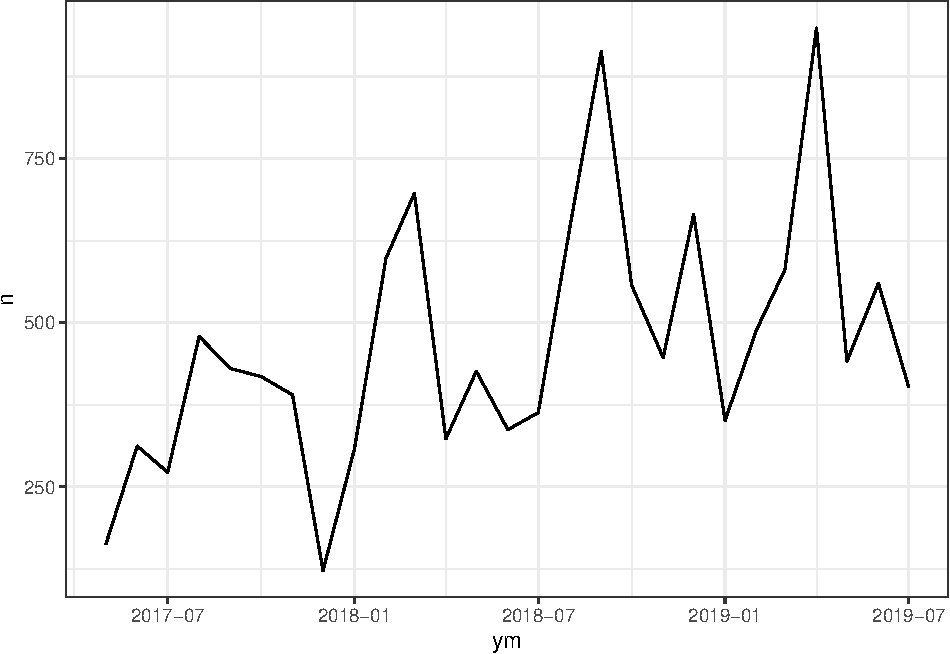
\includegraphics{workshop_topicmodels_files/figure-latex/read-data-1.pdf}

\begin{Shaded}
\begin{Highlighting}[]
\NormalTok{d }\OperatorTok\StringTok{ }
\StringTok{  }\KeywordTok{pull}\NormalTok{(}\StringTok{"wc"}\NormalTok{) }\OperatorTok\StringTok{ }
\StringTok{  }\KeywordTok{summary}\NormalTok{()}
\end{Highlighting}
\end{Shaded}

\begin{verbatim}
##    Min. 1st Qu.  Median    Mean 3rd Qu.    Max. 
##      20      37      60      87     102    2493
\end{verbatim}

\begin{itemize}
\tightlist
\item
  Der Datensatz besteht aus 12,635 Posts.

  \begin{itemize}
  \tightlist
  \item
    Die Variable \texttt{post} enthält den vollen Text des Posts.
  \item
    Die Variable \texttt{author} enthält den Accountnamen, von dem der Post abgegeben wurde.
  \item
    Die Variable \texttt{date} enthält den Tag der Veröffentlichung.
  \item
    Die Variable \texttt{wc} enthält die Zahl der Wörter des Posts.
  \item
    Die Variable \texttt{thread\_title} enthält den Titel des Diskussions-Threads.
  \end{itemize}
\item
  Pro Monat sind zwischen ca. 120 und 1.000 Posts in unserer Stichprobe.
\item
  Typische Posts haben einen Umfang von zwischen 40 und 100 Wörtern (Zur Erinnerung: Sehr kurze Post wurden bereits ausgeschlossen).
\end{itemize}

  \bibliography{book.bib}

\end{document}
